\documentclass[11pt]{article}

% ---------- Packages ----------
\usepackage[margin=1in]{geometry}
\usepackage{amsmath,amssymb}
\usepackage{graphicx}
\usepackage{booktabs}
\usepackage{longtable}
\usepackage{array}
\usepackage[table]{xcolor}
\usepackage{hyperref}
\usepackage{caption}
\usepackage{enumitem}
\usepackage{fancyhdr}
\usepackage{titlesec}
\usepackage[most]{tcolorbox}

\hypersetup{colorlinks=true, linkcolor=blue!50!black, urlcolor=blue!50!black}

\definecolor{assumedcolor}{RGB}{178,34,34}
\definecolor{papercolor}{RGB}{0,102,51}
\definecolor{derivedcolor}{RGB}{0,51,153}
\newcommand{\FROMPAPER}{\textcolor{papercolor}{\textbf{[PAPER]}}}
\newcommand{\DERIVED}{\textcolor{derivedcolor}{\textbf{[DERIVED]}}}
\newcommand{\ASSUMED}{\textcolor{assumedcolor}{\textbf{[ASSUMED]}}}

\newcommand{\usd}{USD}
\newcommand{\tpy}{t/yr}

\setlength{\headheight}{14pt}
\pagestyle{fancy}
\fancyhf{}
\fancyhead[L]{\small Competing plastic-recycling firms --- linear-cost model}
\fancyhead[R]{\small\thepage}
\renewcommand{\headrulewidth}{0.4pt}

\titleformat{\section}{\normalfont\Large\bfseries}{\thesection}{0.8em}{}
\titleformat{\subsection}{\normalfont\large\bfseries}{\thesubsection}{0.8em}{}
\setlength{\parskip}{0.55em}
\setlength{\parindent}{0pt}

\tcbset{
  boxsep=2pt, left=8pt, right=8pt, top=6pt, bottom=6pt,
  colback=blue!4!white, colframe=blue!50!black, fonttitle=\bfseries,
  breakable
}
\newtcolorbox{keybox}[1][]{#1}
\newtcolorbox{cautionbox}[1][]{colback=orange!7!white, colframe=orange!70!black, #1}

\title{\textbf{What Does Feedstock Cost When Three Recycling\\
Technologies Compete for the Same Waste?}\\[0.4em]
\large A game-theory extension of the multilayer-film decision-support paper\\
(linear-cost model, base case and feedstock-scarcity sweep)}
\author{Parth Brahmbhatt --- Avraamidou Lab}
\date{\today}

\begin{document}
\maketitle

% =============================================================================
\begin{keybox}[title={The short version}]
\textbf{The question.} In the multilayer-film paper, one planner decides where
all 8{,}000 t/yr of waste goes. Here we ask what happens if STRAP,
incineration and gasification are three \emph{separate firms} that must compete
to buy that same limited waste. Competition puts an implicit price on the waste,
called $\lambda$ (USD per ton). It is not assumed; it comes out of the model.

\textbf{What we found} (base case, 8{,}000 t/yr):
\begin{itemize}[leftmargin=1.4em,itemsep=0.2em,topsep=0.2em]
  \item \textbf{$\lambda = 175.57$ \usd/ton}, and incineration is the firm that sets it.
  \item STRAP wins the waste first: it takes its full 6{,}000 t/yr because it can
        afford to pay about 6.5 times more per ton than incineration.
        Incineration gets the remaining 2{,}000 t/yr. Gasification gets nothing.
  \item Gasification loses money on every ton it processes, even if the waste is
        free (net margin $-16.69$ \usd/t), so it never enters at any waste volume.
  \item As the available waste changes, the price does not move smoothly. It
        takes only three values: 1{,}137.84, 175.57 or 0 \usd/t, switching at
        6{,}000 and 10{,}000 t/yr.
\end{itemize}

\textbf{What we need from you.} Several inputs are not in the paper and had to
be assumed. The headline price is controlled almost entirely by
\emph{incineration's} numbers, so the three questions that matter most are
\textbf{Q1} (incineration operating cost), \textbf{Q2} (incineration revenue) and
\textbf{Q3} (plant capacities) in Section~\ref{sec:questions}.
\end{keybox}

\vspace{0.4em}
\noindent\textbf{Color key.}
\FROMPAPER\ value taken from the paper;
\DERIVED\ value recovered from the authors' own notebook/spreadsheet (real data,
not printed in the paper);
\ASSUMED\ value with no source, a defensible default that needs your check.

% =============================================================================
\section{The idea in plain words}

\textbf{Three firms, one pile of waste.} Each technology is treated as its own
profit-maximizing firm: \textbf{S} (STRAP), \textbf{W} (incineration) and
\textbf{G} (gasification for energy recovery). They all draw on the same
8{,}000 t/yr of post-industrial multilayer film. Every ton one firm takes is a
ton the others cannot have, and that shared limit is what couples them.
Landfill is not a firm. It is only where each firm's leftover residue goes (at a
fee) and where any unbought waste ends up.

\textbf{The price that clears the market.} Think of an auction for a fixed pile
of waste. Each firm has a \emph{walk-away price}: the most it could pay for one
more ton and still break even on operations. We call this its
\textbf{net margin} $m_i$. The market-clearing price $\lambda$ is the price at
which the firms' total demand just matches the pile. Economically, $\lambda$ is
the price of scarcity: what the waste is worth once firms have to compete for it.

\textbf{Why the outcome is a queue.} In this version every firm's operating cost
is a fixed amount per ton. A firm that earns the same margin on every ton has no
reason to take ``a little'': if the price is below its walk-away price it wants
as much as it can process, and if the price is above, it wants none. So the
firms line up in order of walk-away price, each takes its full capacity, and the
last firm in line, the one only partly filled, sets the price. This is called a
\emph{merit order}, and it is why the answer can be found by simple arithmetic
rather than a numerical solver.

% =============================================================================
\section{What each firm earns per ton}

Each firm's net margin is what is left of a ton's revenue after its operating
cost and the landfill fee on its own residue (the feedstock itself is free in
the base case, $p_{\mathrm{raw}}=0$):
\[
m_i \;=\; \text{revenue}_i \;-\; \text{operating cost}_i \;-\; \text{landfill fee}\times\text{residue fraction}_i .
\]

\begin{table}[h]
\centering
\caption{Net margin per ton of feedstock, \usd/ton. Landfill fee is
60~\usd/t times the residue fraction.}
\label{tab:margins}
\begin{tabular}{@{}lrrrr@{}}
\toprule
Firm & Revenue & $-$ Operating cost & $-$ Landfill on residue & $=$ Net margin $m_i$ \\
\midrule
S\ \ STRAP         & 1{,}468.39 & 311.28 & 19.26 (0.321 t/t) & \textbf{1{,}137.84} \\
W\ \ Incineration  &   259.57   &  75.00 &  9.00 (0.150 t/t) & \textbf{175.57} \\
G\ \ Gasification  &   147.98   & 159.87 &  4.80 (0.080 t/t) & \textbf{$-$16.69} \\
\bottomrule
\end{tabular}
\end{table}

\begin{figure}[h]
\centering
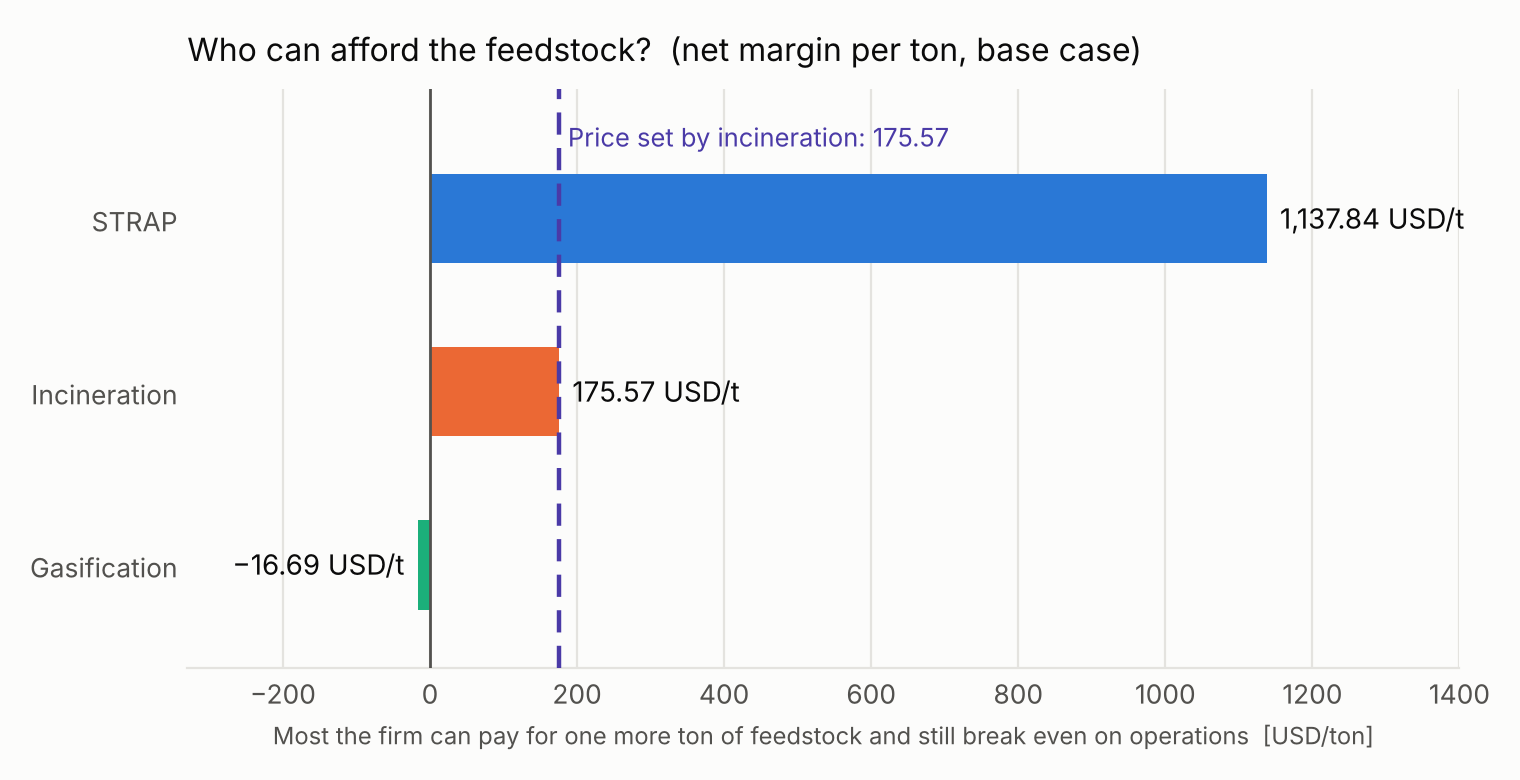
\includegraphics[width=0.88\textwidth]{figures/figL0_margins.png}
\caption{Each firm's walk-away price. The dashed line is the equilibrium price at
8{,}000 t/yr: STRAP is far above it, gasification is below zero, and
incineration sits exactly on it.}
\label{fig:margins}
\end{figure}

Three things stand out. STRAP's margin is large because resin is worth much more
than energy. Incineration earns a thin but positive margin. And gasification's
margin is negative: with the authors' own revenue figure (148 \usd/t) and
operating cost (160 \usd/t), it costs more to run than the energy it produces
is worth, before any feedstock price is even charged.

% =============================================================================
\section{Result at the base case (8{,}000 t/yr)}
\label{sec:base}

Fill the queue in order of margin. STRAP takes its full 6{,}000 t/yr (it would
take more if it could). That leaves 2{,}000 t/yr, which is less than
incineration's 4{,}000 t/yr capacity, so incineration is only partly filled and
is exactly on the margin. Gasification's margin is negative, so it takes nothing.
The price is therefore incineration's walk-away price:
\[
\boxed{\;\lambda^\ast = m_W = 175.57\ \usd/\text{ton}\;}
\]

\begin{table}[h]
\centering
\caption{Base-case equilibrium. Operating profit is margin $\times$ tons; profit
after capital subtracts the annualized capital charge (CRF $=0.1175$).}
\label{tab:base}
\begin{tabular}{@{}lrrlrrr@{}}
\toprule
Firm & Tons/yr & Share & Status & \shortstack{Operating\\profit (\usd/yr)} & \shortstack{Profit after\\capital (\usd/yr)} & \shortstack{Emissions\\(t CO$_2$e/yr)} \\
\midrule
S & 6{,}000 & 75\% & At capacity     & 6{,}827{,}062 &    523{,}742 & 7{,}329 \\
W & 2{,}000 & 25\% & Sets the price  &   351{,}140 & $-$3{,}173{,}860 & 4{,}786 \\
G &       0 &  0\% & Priced out      &         0   & $-$2{,}282{,}998 &       0 \\
\midrule
Total & 8{,}000 & 100\% & & 7{,}178{,}202 & $-$4{,}933{,}116 & 12{,}115 \\
\bottomrule
\end{tabular}
\end{table}

\textbf{How to read $\lambda$.} Every firm pays $p_{\mathrm{raw}}+\lambda$ per
ton of waste, where $p_{\mathrm{raw}}$ is whatever the waste generator charges
(zero here). Raising $p_{\mathrm{raw}}$ lowers $\lambda$ one-for-one, so the
total price a firm actually pays stays at 175.57 \usd/t until $p_{\mathrm{raw}}$
reaches 175.57 and $\lambda$ hits zero. STRAP's \emph{capacity shadow price} is
$\mu_S = m_S-\lambda = 962.27$ \usd/(t/yr): how much STRAP's operating profit
would rise for each extra ton/yr of plant, at an unchanged price.

\begin{cautionbox}[title={Worth knowing: the price depends on incineration existing}]
Capital charges are treated as already paid, because capacities are fixed inputs.
On that basis incineration runs, since it earns 351{,}140 \usd/yr in cash. But
after its \emph{assumed} 30~million \usd{} plant is paid for, it loses 3.2~million \usd/yr, and
only STRAP is profitable. If no incinerator were built at all, STRAP would
still take 6{,}000 t/yr, 2{,}000 t/yr would go unbought, and
$\lambda$ at 8{,}000 t/yr would be \textbf{0}, not 175.57. The headline price
therefore rests on the incinerator being there, which is one more reason
Q1--Q3 matter.
\end{cautionbox}

% =============================================================================
\section{What happens as feedstock availability changes}
\label{sec:sweep}

We re-solved the equilibrium for every availability $Q_{\mathrm{tot}}$ from 0 to
18{,}000 t/yr (207 points, including each switching point and points just on
either side).

\begin{figure}[h]
\centering
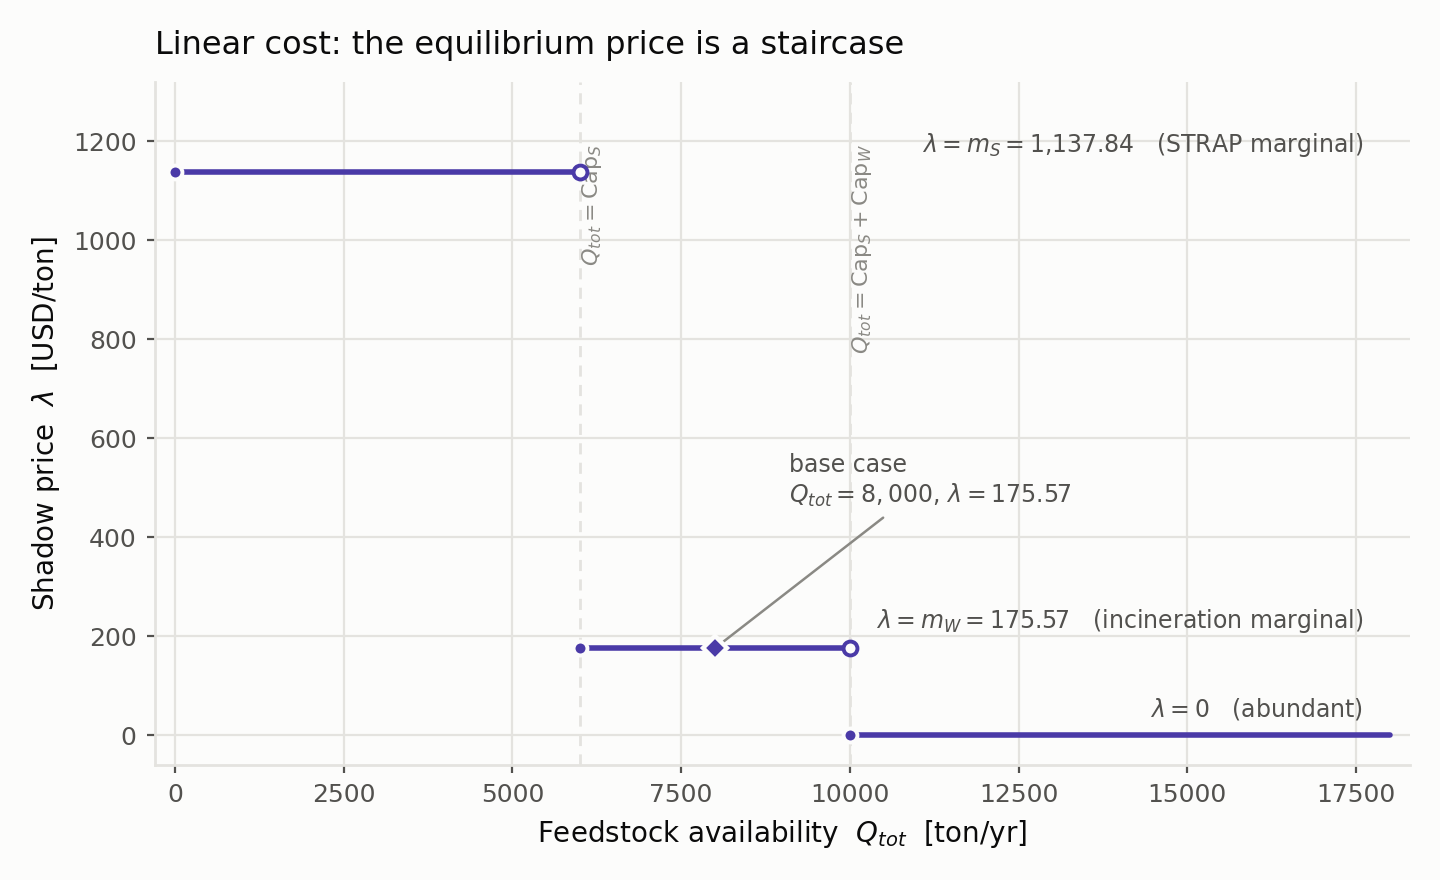
\includegraphics[width=0.88\textwidth]{figures/figL1_lambda_staircase.png}
\caption{Equilibrium price against feedstock availability. It is a staircase:
flat within a regime, with a jump each time the last firm in line changes.}
\label{fig:L1}
\end{figure}

\begin{table}[h]
\centering
\caption{The three regimes.}
\label{tab:regimes}
\begin{tabular}{@{}llrl@{}}
\toprule
Regime & Availability (t/yr) & $\lambda$ (\usd/t) & Who sets the price \\
\midrule
Severe scarcity   & below 6{,}000          & 1{,}137.84 & STRAP \\
Moderate scarcity & 6{,}000 to 10{,}000    &   175.57   & Incineration \\
Abundance         & above 10{,}000         &     0      & Nobody; extra waste is landfilled \\
\bottomrule
\end{tabular}
\end{table}

The switching points are exact: 6{,}000 is STRAP's capacity, and 10{,}000 is STRAP's
plus incineration's. The upper limit is 10{,}000, not the 14{,}000 t/yr of total
installed capacity, because gasification never runs.

\textbf{Exactly at 6{,}000 and 10{,}000 the price is not unique.} At
$Q_{\mathrm{tot}}=6{,}000$ any price from 175.57 to 1{,}137.84 is consistent
with equilibrium, and at 10{,}000 any price from 0 to 175.57. The tables and
figures report the \emph{lowest} consistent price at each of these two points.
So the drop at 6{,}000 should be read as ``just below versus just above,'' not
as a response to a single extra ton. Just above 6{,}000 the price falls by
962.27 \usd/t, an 85\% drop, because the next buyer in line (incineration) values
a ton at roughly one-sixth of what STRAP does.

\begin{figure}[h]
\centering
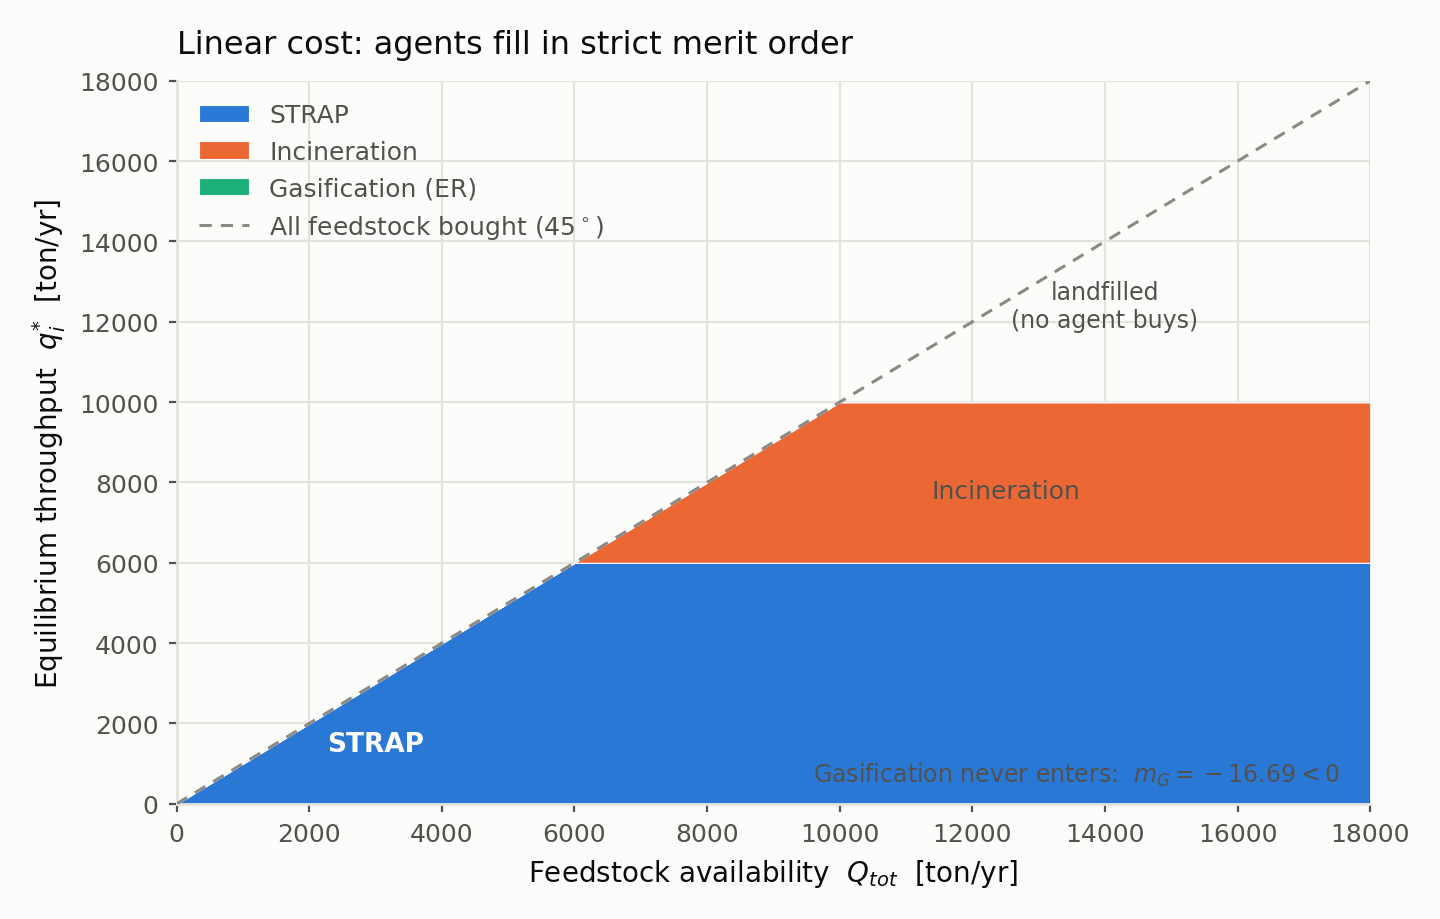
\includegraphics[width=0.88\textwidth]{figures/figL2_allocation.png}
\caption{Who gets the waste. STRAP fills first, then incineration; gasification
never enters. Above 10{,}000 t/yr the gap to the dashed line is waste nobody buys.}
\label{fig:L2}
\end{figure}

\textbf{What this can and cannot tell us.} The order of the firms and the two
switching points are robust: they depend only on how the margins rank and on the
capacities. What the model cannot show is a \emph{gradient}. At 6{,}100 t/yr and
at 9{,}900 t/yr it returns the same price, 175.57. With a constant cost per ton,
the model can describe scarcity regimes but not ``a little scarcer.'' A convex
(rising marginal cost) version would give a sloped price and is the natural next
step.

% =============================================================================
\section{What moves the answer, and what does not}
\label{sec:sensitivity}

At 8{,}000 t/yr the price is simply incineration's margin:
\[
\lambda^\ast \;=\; m_W \;=\; \text{REV}_W - a_W - p_{\mathrm{raw}} - c_{\mathrm{lf}}\,\rho_W
\;=\; 259.57-75.00-0-60\times0.15 \;=\; 175.57 .
\]
That one line explains most of the sensitivity:
\begin{itemize}[leftmargin=1.4em,itemsep=0.2em]
  \item \textbf{Moves it one-for-one:} incineration's revenue and operating cost,
        and the feedstock price $p_{\mathrm{raw}}$.
  \item \textbf{Moves it through the landfill fee:} each extra 0.01 of
        incineration's residue fraction lowers $\lambda$ by 0.60 \usd/t, and each
        extra 10~\usd/t of landfill fee lowers it by 1.50 \usd/t.
  \item \textbf{Does not move it at all:} every STRAP economic number (as long as STRAP's
        margin stays above incineration's, i.e.\ STRAP revenue above about
        506~\usd/t), every gasification number (unless gasification revenue rose
        above about 340~\usd/t, more than double today's), and the capital-recovery
        convention.
  \item \textbf{Moves it in jumps:} the plant capacities. They decide which
        regime 8{,}000 t/yr falls in (Table~\ref{tab:regimes}).
\end{itemize}

% =============================================================================
\section{Questions for Paola}
\label{sec:questions}

These are inputs that are not in the paper, ordered by how much they change the
headline price. The last column shows what $\lambda$ becomes at 8{,}000 t/yr if
the value were different (everything else held at the base case).

{\small
\setlength{\tabcolsep}{4pt}
\renewcommand{\arraystretch}{1.25}
\begin{longtable}{@{}>{\raggedright\arraybackslash}p{0.3cm}>{\raggedright\arraybackslash}p{6.2cm}>{\raggedright\arraybackslash}p{3.4cm}>{\raggedright\arraybackslash}p{4.7cm}@{}}
\toprule
 & \textbf{What we need from you} & \textbf{What we assumed} & \textbf{Effect on $\lambda$ at 8{,}000 t/yr} \\
\midrule
\endhead
\multicolumn{4}{@{}l}{\textbf{Move the headline price directly}}\\*[0.2em]
1 & \textbf{Incineration operating cost.} The workbook records it as zero (incineration is modeled only as an off-take market). Do you have a per-ton figure for this feedstock? & 75 \usd/t, mid-range US waste-to-energy O\&M (typical 60--90) \ASSUMED & 60 gives 190.57; 90 gives 160.57. One-for-one. \\
2 & \textbf{Incineration revenue.} Is \texttt{Cwte}~=~259.57 \usd/t the value of the energy sold per ton burned, and \texttt{Cgas\_pw}~=~110 \usd/t the transfer price for the waste itself? We used 259.57 because an operating firm earns the product value. & 259.57 \usd/t \DERIVED & If 110 were the right revenue, $\lambda$ falls to \textbf{26.0} (about 6.8 times lower). \\
3 & \textbf{Plant capacities.} Is there a defensible single-plant scale for STRAP, and any basis for incineration and gasification capacities? & 6{,}000 / 4{,}000 / 4{,}000 t/yr \ASSUMED & 175.57 while $\mathrm{Cap}_S<8{,}000<\mathrm{Cap}_S+\mathrm{Cap}_W$. 1{,}137.84 if $\mathrm{Cap}_S>8{,}000$; 0 if the two together are below 8{,}000. \\
4 & \textbf{Landfill tipping fee.} The spreadsheet implies 7.836 \usd/t, about 8 times below real Wisconsin gate rates. Is it a tipping fee or a different cost (e.g.\ processing)? & 60 \usd/t \ASSUMED\ (paper: 7.836) & 7.836 gives 183.39. \\
5 & \textbf{Feedstock price.} What should a recycler pay for post-industrial waste? The paper gives it free; the authors' model implies 110 \usd/t in another context; it could even be negative. & 0 \usd/t \ASSUMED & 110 gives 65.57; $-50$ gives 225.57. One-for-one, down. \\
6 & \textbf{Ash/residue fractions.} The workbook records zero ``waste to disposal'' for incineration and gasification. Placeholder, or accounted for elsewhere? & 0.15 and 0.08 t/t \ASSUMED & With zero ash in incineration, 184.57; each extra 0.05 lowers $\lambda$ by 3.00. \\[0.4em]
\midrule
\multicolumn{4}{@{}l}{\textbf{Matter only in other scenarios}}\\*[0.2em]
7 & \textbf{Gasification revenue inputs.} The heat price (0.13 \usd/MJ, i.e.\ 130 \usd/GJ) and heat yield (583 MJ/t) both look unusual individually. Are they in the units the notebook implies? & 147.98 \usd/t \DERIVED & None at 8{,}000 t/yr unless revenue exceeds about 340. It decides whether gasification ever runs: it needs above 164.67 (+11\%) to break even on operations. \\[0.4em]
\midrule
\multicolumn{4}{@{}l}{\textbf{Do not change $\lambda$}}\\*[0.2em]
8 & \textbf{Capital recovery convention.} We used 10\%/20-year discounting (CRF 0.1175); the paper divides by 20 (0.05). Deliberate? & 0.1175 \ASSUMED & None. Changes only profit after capital. \\
9 & \textbf{Emissions units.} Table 8's ``kg CO$_2$-eq/year'' reproduces exactly if the data are really tonnes. Can you confirm the Table 8--10 columns are tonnes? & Tonnes & None. Affects emission totals only. \\
10 & \textbf{Table 8 profit.} We could not rebuild the published 7{,}551{,}142 \usd/yr from the workbook's per-wash CAPEX/OPEX under any single convention (shredder charged once vs.\ twice; wash-2 capital in or out). Which convention produced it? & --- & None. Only a plausibility check. \\
\bottomrule
\end{longtable}
}

% =============================================================================
\section{Limits of this version, and what we checked}
\label{sec:limits}

\textbf{Deliberate simplifications.}
Operating cost is linear (constant per ton), which is what makes the price a
staircase. Product prices, the landfill fee and the feedstock price are fixed:
no firm's actions move a market price. There is no emissions cap (emissions are
reported, never constrained), and capacities are fixed inputs rather than the
result of a capacity-choice game. A convex-cost version is the natural next
step: it would give a smoothly varying price and a unique split of waste among
firms.

\textbf{Two caveats on the base-case profits.}
(i)~STRAP's capital (53.6~million \usd) comes from the 8{,}000 t/yr simulation, but we give
STRAP a 6{,}000 t/yr capacity. Scaling capital down with the usual six-tenths
rule would cut its capital charge from 6.30 to 5.30~million \usd/yr and raise STRAP's
profit after capital from 0.52 to about 1.5~million \usd/yr. This does not touch
$\lambda$. (ii)~The incinerator's 30~million \usd{} capital is assumed, not sourced, and is
what makes it unprofitable after capital (see the box in Section~\ref{sec:base}).

\textbf{How we checked the numbers.}
Every derived number in this report (revenues, margins, capital charges,
emission factors and the base-case results) was re-derived independently from the
raw inputs, without using the model code, and agrees with the code's output.
The 207-point sweep was also recomputed point by point by brute-force search
over prices, and every point matches. All equilibrium conditions hold with a
worst violation of exactly zero (the solution is closed-form, so there is no
iteration error), the price never increases as availability grows, and no two
firms are ever tied on the margin at a swept point.

% =============================================================================
\clearpage
\appendix
\section{Parameters}

{\small
\setlength{\tabcolsep}{4pt}
\renewcommand{\arraystretch}{1.15}
\begin{longtable}{@{}>{\raggedright\arraybackslash}p{8.3cm}>{\raggedright\arraybackslash}p{5.2cm}l@{}}
\caption{Inputs, by firm. Units are per ton of feed unless stated.}\label{tab:params}\\
\toprule
\textbf{Parameter} & \textbf{Value} & \textbf{Source} \\
\midrule
\endfirsthead
\toprule
\textbf{Parameter} & \textbf{Value} & \textbf{Source} \\
\midrule
\endhead
\multicolumn{3}{@{}l}{\textit{Feedstock}}\\*
Base availability & 8{,}000 t/yr & \FROMPAPER \\
Mass fractions PE / PET / N6 / EVOH & 0.60 / 0.20 / 0.10 / 0.10 & \FROMPAPER \\
\addlinespace
\multicolumn{3}{@{}l}{\textit{S --- STRAP (frozen to the paper's best pathway: wash 1 PE/PCE, wash 2 EVOH/GBL)}}\\*
Yield (PE and EVOH recovered) & 0.97 & \FROMPAPER \\
Resin prices, PE / EVOH & 1{,}173 / 8{,}100 \usd/t & \FROMPAPER \\
Revenue per ton of feed & 1{,}468.39 \usd/t & \DERIVED \\
Residue fraction (PET + N6 + losses) & 0.321 & \DERIVED \\
Operating cost & 2{,}490{,}259 \usd/yr at 8{,}000 t/yr, i.e.\ 311.28 \usd/t & \DERIVED \\
Installed capital (wash 1 + wash 2 + shredder) & 53{,}645{,}274 \usd & \DERIVED \\
Process emissions & 1.194 t CO$_2$e/t & \DERIVED \\
Capacity & 6{,}000 t/yr & \ASSUMED \\
\addlinespace
\multicolumn{3}{@{}l}{\textit{W --- Incineration}}\\*
Revenue (energy value) & 259.57 \usd/t & \DERIVED \\
Operating cost & 75 \usd/t & \ASSUMED \\
Residue (ash) fraction & 0.15 & \ASSUMED \\
Installed capital & 30{,}000{,}000 \usd & \ASSUMED \\
Process emissions & 2.38 t CO$_2$e/t & \DERIVED \\
Capacity & 4{,}000 t/yr & \ASSUMED \\
\addlinespace
\multicolumn{3}{@{}l}{\textit{G --- Gasification for energy recovery}}\\*
Revenue: 583.33 MJ/t $\times$ 0.13 \usd/MJ $+$ 724.37 kWh/t $\times$ 0.0996 \usd/kWh & 147.98 \usd/t & \DERIVED \\
Operating cost & 159.87 \usd/t & \DERIVED \\
Residue (ash/char) fraction & 0.08 & \ASSUMED \\
Annualized capital ($15{,}749.6\times\mathrm{Cap}^{0.6}$; already annualized by the authors) & 2{,}282{,}998 \usd/yr & \DERIVED \\
Process emissions & 1.07 t CO$_2$e/t & \DERIVED \\
Capacity & 4{,}000 t/yr & \ASSUMED \\
\addlinespace
\multicolumn{3}{@{}l}{\textit{Shared}}\\*
Feedstock price $p_{\mathrm{raw}}$ & 0 \usd/t & \ASSUMED \\
Landfill tipping fee $c_{\mathrm{lf}}$ & 60 \usd/t & \ASSUMED \\
Capital recovery factor (10\%, 20 years) & 0.1175 per year & \ASSUMED \\
Landfill emission factor (0.0816 plus a 9.2-mile haul) & 0.0865 t CO$_2$e/t & \DERIVED \\
\bottomrule
\end{longtable}
}

\section{Where the harder numbers come from}

\textbf{STRAP capital and operating cost.} The paper prints neither. They come
from the authors' BioSTEAM results for the best pathway under energy scenario 1.
Capital is $35{,}957{,}532$ (wash 1) $+\,14{,}557{,}669$ (wash 2) $+\,3{,}130{,}073$
(shredder). Operating cost is $941{,}557+479{,}709+1{,}068{,}992$ \usd/yr. The
shredder is counted once; the authors' workbook charges it to both washes.
The process emission factor is built from the per-resin factors (1.1326 for PE,
2.1661 for EVOH, 0.5575 for the shredder, all t CO$_2$e per ton of resin),
scaled to the 4{,}656 t/yr of PE and 776 t/yr of EVOH recovered at 8{,}000 t/yr.

\textbf{Incineration.} The paper does not model incineration as a facility. The
planner \emph{sells} waste to it at 110 \usd/t (\texttt{Cgas\_pw}), and the
workbook records its capital and operating cost as zero. Because the game needs
incineration to be an operating firm, we used \texttt{Cwte} = 259.57 \usd/t for
revenue and assumed the operating cost and capital (Q1, Q2).

\textbf{Gasification.} Revenue is built from the authors' own yields and prices.
Two inputs look off on their own: the heat price (130 \usd/GJ) is roughly ten
times typical industrial heat prices, and the heat yield (583 MJ/t) is far below
the heating value of plastic (30--40 GJ/t). We cannot say which way correcting
them would move revenue, because the two errors, if they are errors, push in
opposite directions. This is Q7. Capital is already annualized in the authors'
spreadsheet, so the capital recovery factor is not applied again.

\textbf{Emissions units.} Table 8 of the paper labels the landfill-only emissions
``652.80 kg CO$_2$-eq/year.'' That is exactly $0.0816\times 8{,}000$, and the
underlying column is in tonnes, so we read the label as an error and apply no
unit correction (Q9). Two small consistency notes: the landfill factor used for
residue includes a 9.2-mile haul (0.0865), while incineration's process factor
excludes its 151-mile haul; including it would add about 1.3\% to system
emissions.

\textbf{Comparison with the paper.} Routing all 8{,}000 t/yr to STRAP alone gives
an operating profit of 9{,}102{,}749 \usd/yr here. The paper's Table 8 maximum-profit
figure is 7{,}551{,}142 \usd/yr, but that figure is after capital charges and
includes a gasification pathway, so the two are \emph{not} like-for-like. The
agreement in order of magnitude is only a rough plausibility check, not a
validation.

\section{The math, for reference}

Each firm $i\in\{S,W,G\}$ chooses throughput $q_i\ge 0$ (ton/yr) to maximize
\[
\pi_i \;=\; m_i\,q_i \;-\; \mathrm{ACC}_i,
\qquad
m_i \;=\; \sum_k P_k\,\eta_{ik} \;-\; a_i \;-\; p_{\mathrm{raw}} \;-\; c_{\mathrm{lf}}\,\rho_i ,
\]
where $P_k$ are product prices, $\eta_{ik}$ the yield of product $k$ per ton of
feed, $a_i$ the operating cost per ton, $\rho_i$ the residue fraction and
$\mathrm{ACC}_i$ the annualized capital charge (a constant, so it does not affect
$q_i^\ast$). The firms are linked by one shared constraint:
\[
q_i \le \mathrm{Cap}_i \ \ (\text{multiplier } \mu_i),
\qquad
\sum_{j} q_j \le Q_{\mathrm{tot}} \ \ (\text{multiplier } \lambda).
\]
Because the constraint is shared, this is a \emph{generalized} Nash game. We solve for the
\emph{variational equilibrium}, in which every firm faces the same $\lambda$,
the natural concept for a market with a single clearing price. Stacking the
firms' optimality (KKT) conditions gives
\begin{align*}
0 \le q_i &\;\perp\; \lambda+\mu_i-m_i \ge 0, \\
0 \le \mu_i &\;\perp\; \mathrm{Cap}_i-q_i \ge 0, \\
0 \le \lambda &\;\perp\; Q_{\mathrm{tot}}-\textstyle\sum_j q_j \ge 0 .
\end{align*}
The term $\lambda+\mu_i-m_i$ does not depend on $q_i$, which is the formal
statement that cost is linear. Each firm's best response is therefore a step:
\[
q_i(\lambda)=
\begin{cases}
\mathrm{Cap}_i & m_i>\lambda,\\
0 & m_i<\lambda,\\
\text{anything in }[0,\mathrm{Cap}_i] & m_i=\lambda .
\end{cases}
\]
Aggregate demand $D(\lambda)=\sum_{i:\,m_i>\lambda}\mathrm{Cap}_i$ is a step function, and the
equilibrium price is the lowest $\lambda\ge 0$ with $D(\lambda)\le Q_{\mathrm{tot}}$;
the firm exactly at $\lambda$, if any, absorbs the remainder. Firms strictly above
it run at capacity, and firms strictly below take nothing. If two firms ever tied
on margin, the price would still be unique but the split between them would not.
That does not happen in the base case or anywhere in the sweep.
System emissions are $\sum_i e_i q_i^\ast + g_{\mathrm{lf}}\,(Q_{\mathrm{tot}}-\sum_i q_i^\ast)$,
reported only and never constrained.

\medskip
\noindent\textbf{Source paper.} Mu\~{n}oz-Briones, Ikegwu, Martinez, Granger, Van Lehn,
Zavala, Huber and Avraamidou, \emph{Decision support for circular economy waste
management of mixed plastic streams: A case study on post-industrial multilayer
films.}

\noindent\textbf{Code.} \texttt{Code/linear\_model.py} (solver and sweep) and
\texttt{Code/plots\_linear.py} (figures); full sweep output in
\texttt{Code/results/linear\_sweep\_q\_tot.csv}.

\end{document}
